\section{Theoretical Analysis}
\label{sec:theoretical}

\noindent \par In this section, the circuit shown in figure \ref{fig:1} is analysed theoretically.
\par The following analysis will be made considering the ideal model of an OP-AMP, where its gain is infinite, with an infinite input impedance and 0 output impedance. Pratically speaking an OP-AMP has different values for the properties refered above. These are the most important differences but, of course, they aren't the only ones. This differences will be talked about again when we compare the results and will also help to explain the differences encountered in Octave and NGspice.  
\par This circuit will behave as a non-inverting amplifier and as a band-pass filter. The components responsible for this last feature are the capacitors, since the lower and higher cut off frequencies are calculated from this components like it will be shown below.

\subsection{First Point}

\noindent \par Our theoretical analysis starts by computing the gain and the input and output impedances at central frequency.
\par First we have to calculate the central frequency and for that we'll have to discover the lower and higher cut off frequencies, those will be the poles, using the characteristic equations. The formulae are,

\begin{equation}
	w_{CutOff} = \frac{1}{R1C1}
\end{equation}

\begin{equation}
	w_{CutOff} = \frac{1}{R2C2}
\end{equation}

\par As expected, the highest value will be the high cut off frequency, $w_H$, and the lowest will be the low cut off frequency, $w_L$. Then to discover the central frequency, $w_0$, we use 

\begin{equation}
	w_{0} = \sqrt{w_L w_H}
\end{equation}

\par Since we want a central frequency of $f_0 = 1000 Hz$ ($w_0 = 2000\pi rad/s$), and from the previous equations we get the following relation

\begin{equation}
	2000\pi = \frac{1}{\sqrt{R1C1R2C2}}
\end{equation}

\par We can now choose the best values for the resistors and capacitors to get the smallest frequency deviation. We found that using a capacitor of 220nF and a parallel of capacitors of 220 for C2 and C1, respectively, and resistors of $1k\Omega$, would get the best results.

\vspace{5mm}
\begin{table}[H]
	\centering
	\begin{tabularx}{0.9\textwidth} {
 	    | >{\raggedright\arraybackslash}X
  	    | >{\raggedleft\arraybackslash}X | }
	\hline
	\input{../mat/frequencias_tab.tex}
	\end{tabularx}
	\caption{All frequencies computed [rad/s]}
	\label{tab:currents}
\end{table}
\vspace{5mm}

\par Now since we know the central frequency we can calculate the gain at that frequency knowing the transfer function. We now show the formula used, the explanation of this formula will be made in the next subssection when we deduce the tranfer function.

\begin{equation}
	Gain = |\frac{1}{1 + j R2 C2 w_0} \frac{j R1 C1 w_0}{1 + j R1 C1 w_0} (1 + \frac{R3}{R4})| 
\end{equation}

\begin{equation}
	Gain_{dB} = 20 log_{10}(Gain)
\end{equation}

\vspace{5mm}
\begin{table}[H]
	\centering
	\begin{tabularx}{0.9\textwidth} {
 	    | >{\raggedright\arraybackslash}X
  	    | >{\raggedleft\arraybackslash}X | }
	\hline
	\input{../mat/ganhos_tab.tex}
	\end{tabularx}
	\caption{Computed Gains}
	\label{tab:currents}
\end{table}
\vspace{5mm}
 
\par To calculate the input and output impedances we just had to analise the circuit and knowing the input and output impedance of the OP-AMP we determine that the input impedance is equal to the impedance of R1 in series with C1 and the output impedance is equal to the impedance of R2 in parallel with C2.

\begin{equation}
	Z_I = R1 + \frac{1}{j w_0 C2}
\end{equation}

\begin{equation}
	Z_o = \frac{R2}{1 + j w_0 C2 R2}
\end{equation}

\begin{table}[H]
	\centering
	\begin{tabularx}{0.9\textwidth} {
 	    | >{\raggedright\arraybackslash}X
  	    | >{\raggedleft\arraybackslash}X | }
	\hline
	\input{../mat/impedancias_tab.tex}
	\end{tabularx}
	\caption{Computed impedances [$\Omega$]}
	\label{tab:currents}
\end{table}
\vspace{5mm}

\par Now lets analise the frequency response of the circuit, and for that, we'll deduce the tranfer function of the circuit.
 
\subsection{Second Point}

\par Knowing that it is a non-inverting amplifier we know the following relation

\begin{equation}
	\frac{v_6}{v_3} = 1 + \frac{R3}{R4}
\end{equation}

\par We still don't have a relation between $v_0$ and $v_I$. To do that we have to relate them with $v_6$ and $v_3$. 
\par Lets find a relation between $v_0$ and $v_6$, applying the voltage divider we have

\begin{equation}
	v_o = \frac{\frac{1}{jwC2}}{\frac{1}{jwC2 + R2}}v_6 = \frac{1}{1 + jR2C2w}
\end{equation}

\par Now to find a relation between $v_3$ and $v_I$, we'll also apply the voltage divider, 

\begin{equation}
	v_3 = \frac{R1}{\frac{1}{jwC1 + R1}}v_I = \frac{jwR1C1}{1 + jR1C1w}v_I
\end{equation}

\par Now that we have the relations that we needed and knowing that $s=jw$, we can combine the last three equations to get

\begin{equation}
	\frac{v_o}{v_I} = T(s) = \frac{1}{1 + R2 C2 s} \frac{s R1 C1}{1 + s R1 C1} (1 + \frac{R3}{R4})
\end{equation}

\par This was the formula used to get the gain at the central frequency in the previous subsection. Doing $T_{dB}(s) = 20log_{dB}(|T(s)|)$ and $\phi = arg(T(s))$, we can plot for frequencies ranging from 10 Hz to 100MHz. We can see in the following figures this ploted in a logarithmic scale.

\begin{figure}[H] 
	\centering
	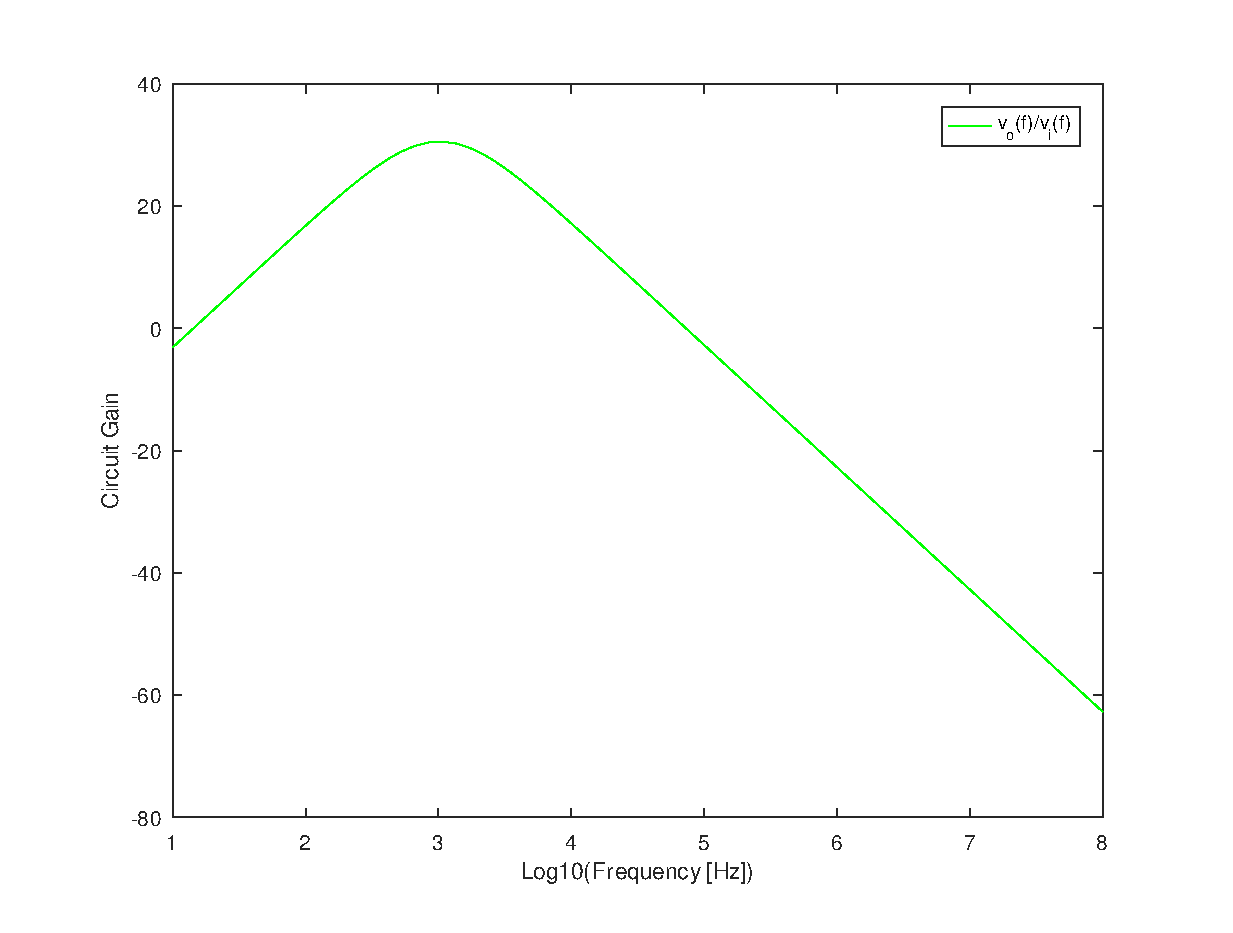
\includegraphics[width=0.75\linewidth]{teoria.eps}
	\caption{Frequency response [dB] ($\frac{V_o(f)}{V_I(f)}$)}
\end{figure}

\begin{figure}[H] 
	\centering
	\includegraphics[width=0.75\linewidth]{fase.eps}
	\caption{Frequency response [degrees]}
\end{figure}

\par To conclude this theoretical analysis we show now the frequency and gain deviation, the cost and the theoretical Merit and we also show the values of the components used.

\vspace{5mm}
\begin{table}[H]
	\centering
	\begin{tabularx}{0.9\textwidth} {
 	    | >{\raggedright\arraybackslash}X
  	    | >{\raggedleft\arraybackslash}X | }
	\hline
	\input{../mat/componentes_tab.tex}
	\end{tabularx}
	\caption{Values of the components used ([$\Omega$],[F])}
	\label{tab:currents}
\end{table}
\vspace{5mm}

\vspace{5mm}
\begin{table}[H]
	\centering
	\begin{tabularx}{0.9\textwidth} {
 	    | >{\raggedright\arraybackslash}X
  	    | >{\raggedleft\arraybackslash}X | }
	\hline
	\input{../mat/final_tab.tex}
	\end{tabularx}
	\caption{Frequency and gain deviation, cost and merit}
	\label{tab:currents}
\end{table}

\par It's important to note that the value for the resistor three was obtained using three resistor of $100k\Omega$, two in parallel with one in series.

\vspace{5mm}

